Elise camina diagonalmente desde una esquina de una plaza cuadrada a la otra.
La longitud de cada lado de la plaza es 50 metros.

\textbf{¿Cuál es la distancia diagonal a través de la plaza?}\\
\textit{Redondea tu respuesta a la décima de metro más cercana.}


\begin{solutionbox}{13cm}
    Sea $x$ la distancia diagonal que Elise caminó a través de la plaza.
    \begin{figure}[H]
        \centering
        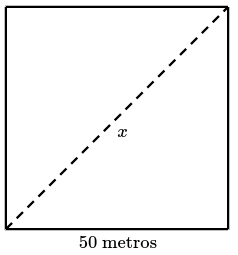
\includegraphics[width=0.2\linewidth]{../images/proverb_pitagoras_11.png}
        \caption{}
        \label{fig:proverb_pitagoras_11}
    \end{figure}
    Podemos usar el teorema de Pitágoras para obtener $x$.
    La ecuación del teorema de Pitágoras es:
    \[c^2=a^2+b^2\]
    donde $a$ y $b$ son las longitudes de los dos catetos del triángulo y $c$ es la longitud de la hipotenusa.
    En este caso, $a=50$, $b=50$ y $c=x$.
    \begin{align*}
        x^2 & =50^2+50^2    \\
        x^2 & =5,000        \\
        x   & =\sqrt{5,000} \\
        x   & \sim 70.7
    \end{align*}
    La distancia diagonal a través de la plaza es aproximadamente 70.7 metros.
\end{solutionbox}